\documentclass[11pt]{article}

\usepackage{a4wide}
\usepackage[utf8]{inputenc}
\usepackage[russian]{babel}
\usepackage{graphicx}
\usepackage{amsmath}
\usepackage{amsfonts}
\usepackage{amssymb}
\usepackage{subcaption}
\usepackage{upgreek}
\usepackage{dsfont}
\begin{document}
	
	\thispagestyle{empty}
	
	\begin{center}
		\ \vspace{-3cm}
		
		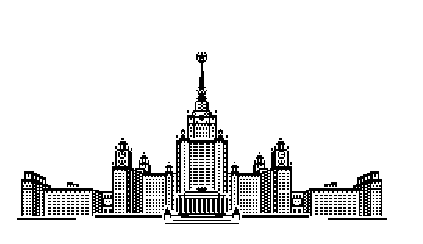
\includegraphics[width=0.5\textwidth]{msu.eps}\\
		{\scshape Московский государственный университет имени М.~В.~Ломоносова}\\
		Факультет вычислительной математики и кибернетики\\
		Кафедра системного анализа
		
		\vfill
		
		{\LARGE Курсовая работа}
		
		\vspace{1cm}
		
		{\Huge\bfseries <<Динамические системы с дискретным временем>>}
	\end{center}
	
	\vspace{1cm}
	
	\begin{flushright}
		\large
		\textit{Студент 315 группы}\\
		А.\,В.~Бабаев
		
		\vspace{5mm}
		
		\textit{Руководитель практикума}\\
		Д.\,А.~ Алимов
	\end{flushright}
	
	\vfill
	
	\begin{center}
		Москва, 2021
	\end{center}
	
	\newpage
	\tableofcontents
	\newpage
	
	{\vspace*{-2cm} \hspace*{-1cm}\section{Постановка задачи}}

	{\hspace{0.4cm}Исследовать системы:}
	\begin{equation}
	 u_{t+1} = ru_t(8 - u_t^3), \quad 0 < u_t < 2  
	 \label{eq:ref1}
	\end{equation}
	\begin{equation}
	 u_{t+1} = ru_t(8 - u_{t-1}^3), \quad 0 < u_t < 2
	 \label{eq:ref2}
	\end{equation}
	
	\begin{itemize}
		\item [1)]{Найти неподвижные точки и исследовать их на устойчивость.}
		\item [2)]{Доказать, что имеется цикл длины 2.}
		\item [3)]{Найти циклы длины 3 и построить бифуркационную диаграмму в зависимости от значения параметра ($r > 0$).}
		\item [4)]{Построить зависимость показателя Ляпунова от значения параметра($r > 0$).}
		\item [5)]{Для систем с запаздыванием построить бифуркационную диаграмму, построить инвариантную кривую в случае существования бифуркации Неймарка-Сакера.}
	\end{itemize}	
	\newpage
	
	{\vspace*{-2cm} \hspace*{-1cm}\section{Исследование системы (\ref{eq:ref1})} }
	{\subsection{Нахождение неподвижных точек}}
	{\hspace*{-0.8cm} \textbf{Определение 2.1.} Точка $U_* \in \mathds{R}$ называется неподвижной точкой системы $u_{t+1} = f(u_t), u_t \in \mathds{R}, f : \mathds{R} \rightarrow \mathds{R}$, если $u_* = f(u_*).$ }
	{Воспользовавшись определением, можно определить все неподвижные точки. Уравнение будет иметь вид:}
	\[ u = ru(8 - u^3)\]
	{Решив его, мы получим 2 неподвижные точки, а именно: $u_1^*=0,u_2^*=(\frac{8r - 1}{r})^{1/3}$}
	
	{\subsection{Исследование характера неподвижных точек}}
	{\hspace*{-0.8cm} \textbf{Определение 2.2.}(Определение устойчивости по Ляпунову). Неподвижная точка $u_*$ отображения $u \rightarrow f(u;r), u \in \mathds{R}, r \in \mathds{R}^m$ называется устойчивой по Ляпунову, если для любого положительного $\varepsilon$ найдется отвечающее ему число $\delta > 0$ такое, что для любой точки $u_0$ из $\delta$-окрестности точки $u_*$ вся траектория системы $u_t, t = 0,1,2,..$ содержится в $\varepsilon$-окрестности точки $u_*$. В противном случае неподвижная точка называется неустойчивой.}

	{\hspace*{-0.8cm} \textbf{Определение 2.3.} Если $u_*$-устойчива по Ляпунову неподвижная точка отображения $U \rightarrow f(u;r), u \in \mathds{R}, r \in \mathds{R}^m$ и, кроме того, $\lim_{t\to\infty} f(u_t) = u_*$, то $u_*$ называется асимптотически устойчивой по Ляпунову.}
	\newline
	{Для исследования точек на устойчивость нам понадобится следующее утверждение:}
	\newline
	\newtheorem{theorem}{Теорема}
	\begin{theorem}
		{Пусть $u_*$ - неподвижная точка системы $u_{t+1} = f(u_t)$, и $f$ обратима в некоторой окрестности точки $u_*$. Тогда если $|f_u(u_*)| < 1$ то точка $u_*$ асимптотически устойчива, если $|f_u(u_*)| > 1$, то она неустойчива. В случае $|f_u(u_*) = 1|$ требуется дальнейшее исследование.}
	\end{theorem}
	{Доказательство. Пусть $|f_u(u^*)| < 1$--- и пусть $u$ принадлежит малой окрестности $u*$. Так как:}
	\[lim_{u \to u^*} \frac{|f(u) - f(u^*)|}{|u - u^*|} = |f_u(u^*)|\]
	{поэтому существует такая окрестность $u^*$, что}
	\[ \frac{|f(u) - f(u^*)|}{|u - u^*|} \leq a \]
	{для всех $u$ из этой окрестности; здесь a --- некоторое число, такое что $|f_u(u^*)| \leq a < 1.$ Таким образом, $f(u)$ остается в той же окрестности, что и $u$, и, кроме того, ближе к неподвижной точке $u^*,$ и по крайней мере, на множитель a. Отсюда следует, что}
	\[ |f(f(u)) - f(f(u^*))| \leq a|f(u) - f(u^*)| < a^2|u - u^*|, \]
	{или, по индукции,}
	\[ |f^{(k)}(u) - u^*| =|f(f^{(k - 1)}(u)) - f(f^{(k - 1)}(u^*))|\leq a|f^{(k - 1)}(u) - f^{(k - 1)}(u^*)| \leq a^k|u - u^*|,\]
	{где $f^k$ означает $k$-ую суперпозицию отображения $f$. Таким образом мы доказали, что последовательность $f^{(k)}(u)$  будет сходится к $u^*$, то есть является асимптотически устойчивой. Вторая часть утверждения доказывается сходным образом.}
	\newline
	\newline
	{Теперь исследуем $f(u,r)^{'}_{u} = 8r - 4u^3$ в окрестностях найденных ранее неподвижных точек $u_1^*=0,u_2^*=(\frac{8r - 1}{r})^{1/3}$.}
	\begin{itemize}
		\item [1.] {При $u^*_1 = 0$:}
		\[ lim_{u \to 0}|f(u,r)^{'}_u| = lim_{u \to 0}| 8r - 4u^3| = 8r.\]
		{Можно выделить следующие случаи:}
		\newline
		{1) $r \in (0, \frac{1}{8}) \Rightarrow |f(u^*_1, r)| < 1 \Rightarrow$ точка $u^*_1 = 0\ \--$  асимптотически устойчива.}
		\newline
		{2) $r = \frac{1}{8} \Rightarrow |f(u^*_1, r)| = 1 \Rightarrow $ необходимы дополнительные исследования.}
		\newline
		{3) $r \in (\frac{1}{8}, \infty) \Rightarrow |f(u^*_1, r)| > 1 \Rightarrow $ точка $u^*_1 = 0\ \--$ является неустойчивой.}
		\item [2.] {При $u^*_2 = (\frac{8r - 1}{r})^{1/3}$:}
		\[ lim_{u \to (\frac{8r - 1}{r})^{1/3}}|f(u,r)^{'}_u| = lim_{u \to (\frac{8r - 1}{r})^{1/3}}| 8r - 4u^3| = |8r - 32 + \frac{4}{r}|.\]
			\newline
		{1) $r \in (\frac{1}{8},\frac{31}{16} - \frac{7 \sqrt{17}}{16}) \cup (\frac{7\sqrt{17}}{16} + \frac{31}{16},4 )\Rightarrow |f(u^*_1, r)| < 1 \Rightarrow$ точка $u^*_2 = (\frac{8r - 1}{r})^{1/3}\ \--$  асимптотически устойчива.}
		\newline
		{2) $r = \frac{1}{8} \Rightarrow |f(u^*_1, r)| = 1 \Rightarrow $ необходимы дополнительные исследования.}
		\newline
		{3) $r \in (0,\frac{1}{8}) \cup (\frac{31}{16} - \frac{7\sqrt{17}}{16},\frac{31}{16} + \frac{7\sqrt{17}}{16}) \cup (4,\infty) \Rightarrow |f(u^*_1, r)| > 1 \Rightarrow $ точка $u^*_1 = 0\ \--$ является неустойчивой.}
		
	\end{itemize}
	{\subsection{Построение бифуркационной диаграммы}}
	{Введем необходимые определения:}
	\newline
	{Рассмотрим дискретную динамическую систему, определяемую отображением $f$:}
	\[u \rightarrow f(u)=f(u;r), \quad u \in U \subset X, \ r \in \mathds{R}, \ f: U \rightarrow U, \]
	{где множество $X \subset \mathds{R}^n$}
	\newline
	{\textbf{Определение 2.4.} Множество всевозможных состояний $u_t$ называется пространством состояний(или фазовым пространством) исходной системы.}
	\newline
	{\textbf{Определение 2.5.}Множество точек $u_t, t = 0,1,...$ называется траекторией(или орбитой) исходной системы, порожденной отображением $f$.}
	\newline
	{\textbf{Определение 2.6.} Динамическая система $u \rightarrow f(u)$ называется топологически эквивалентной в области $U \subset X$ динамической системе $v \rightarrow g(v)$ в области $V \subset X$, если существует гомеоморфизм $h: X \rightarrow X, h(U) = V$, отображающий орбиты первой системы в $U$ на орбиты второй системы в $V$, сохраняя ориентацию во времени.}
	\newline
	{\textbf{Определение 2.7.} Появление топологически неэквивалентных фазовых портретов при изменении вектора параметров рассматриваемой динамической системы называется бифуркацией.}
	\newline
	{\textbf{Определение 2.8.} Бифуркационной диаграммой динамической системы называется разбиение пространства параметров, индуцированное отношением топологической эквивалентности вместе с фазовым портретами для каждого элемента разбиения.}
	\newline
	{Построим бифуркационную диаграмму для системы (1). Введем оси координат, такие что на оси абсцисс отмечается значение параметра $r$, а на оси ординат предельное значение $u_t$ при $е \rightarrow +\infty$. Выберем стартовое значение параметра $r = 0.03 $. Будем увеличивать его с шагом $\delta r = 0.003 $. При каждом фиксированном $r$ выберем произвольную начальную точку $u_0$, например, $u_0 = 0.1$, и проитерируем систему (1) $n = 300$ раз, и выведем последние 150 итераций(для стабилизации системы): }
	\begin{center}
		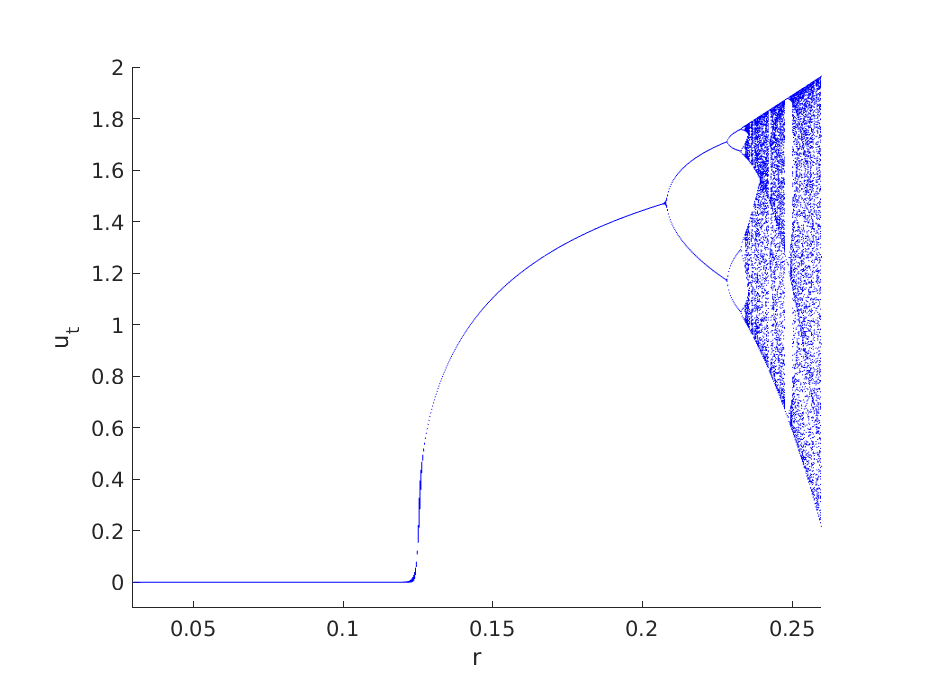
\includegraphics[width=0.7\textwidth]{bifur.eps}\\
		{Рис. 1. Бифуркационная диаграмма для системы (1) при $r \in [0.03, 0.2566]$}
	\end{center}
	{Предельно допустимое значение $r$:}
	\[0 < ru(8 - u^3) < 2\]
	{Возьмем производную по $u$ функции $f(u,r) = ru(8 - u^3)$ и найдем экстремальную точку. $f_u = 8r - 4ru^3 = 0 \rightarrow u = 2^{1/3}$. Решим уравнение $f(2^{1/3},r) = 2.$ Получим, что $r = \frac{1}{2^{1/3}3} = 0.2645.$ Значит этом $r$ достигается предельное значение для исходной функции.}
	\begin{center}
		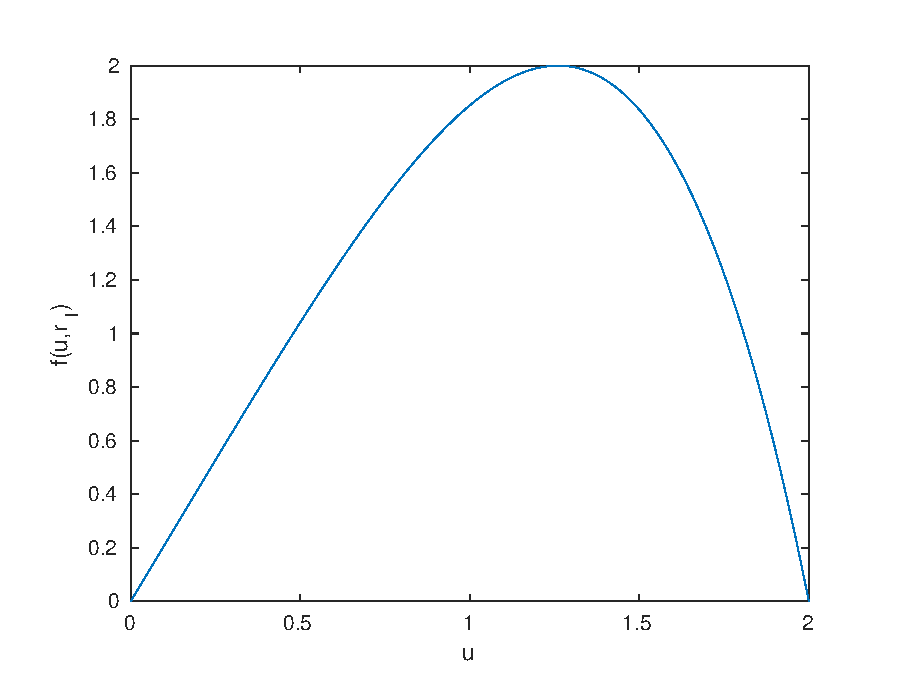
\includegraphics[width=0.7\textwidth]{lim_r.eps}\\
		{Рис. 2. Демонстрация значений функции при $r = 0.2566$}
	\end{center}
	{\subsection{Исследование на наличие циклов длины 2 и 3}}
	{\textbf{Определение 2.9.} Циклом длины $k$ называется набор попарно различных точек $u_1, u_2,\ldots u_k:$}
	\[f(u_1) = u_2, f(u_2) = u_3, \ldots, f(u_k-1) = u_k, f(u_k) = u_1. \]
	{Замечание 2.1. Любая точка цикла является неподвижной точкой отображения $f^{(k)}(u).$}
	\newline
	{\textbf{Определение 2.10.} Упорядочиванием множества натуральных чисел по Шарковскому назовем упорядочивание натуральных числел по следующему порядку:}
	\[3 \succ 5 \succ 7 \succ \ldots \succ \]
	\[\succ 2\cdot3 \succ 2\cdot5 \succ 2\cdot7 \succ \ldots \succ \]
	\[\succ 2^2\cdot3 \succ 2^2\cdot5 \succ 2^2\cdot7 \succ \ldots \succ \]
	\[\succ 2^3\cdot3 \succ 2^3\cdot5 \succ 2^3\cdot7 \succ \ldots \succ \]
	\[\succ \ldots \succ 2^3 \succ 2^2 \succ 2 \succ 1. \]
	
	\begin{theorem}
		{(Шарковский). Пусть $f: \mathds{R} \rightarrow \mathds{R}$--- непрерывное отображение, и пусть $f$ имеет цикл длины $k$. Тогда система имеет цикл длины $m$ для всех таких $m$, что $k \succ m$ в смысле порядка по Шарковскому.}
	\end{theorem}
	{Для нахождения циклов длины 2 найдем неподвижные точки уравнения $f(f(u)) = u,$ отличные от неподвижных точек функции $f(u)$.}
	\newline
	{Из замечания 2.1 следует, что для нахождения цикла длины k нужно найти решение системы:}
	\[ \begin{cases}
	f^{(k)}(u) = u\\
	\frac{df^{(k)}(u)}{du} = 1.
	\end{cases}\]
	{Таким образом, для нахождения циклов длин 2 и 3 необходимо решить соответствующую систему при $k = 2$ и $k = 3$ соответственно.}
	\[ \begin{cases}
	f^{(2)}(u) = u\\
	\frac{df^{(2)}(u)}{du} = 1.
	\end{cases}\]
	{Решить исходную систему аналитически трудно, учитывая наличие степени куба. Поэтому, решение будет проделано численно при помощи возможностей платформы MatLab. Решив эту систему численно, при помощи функции $solve$, которая позволяет решать системы подобного вида. Получим, что цикл длины 2 будет зарождаться при $u \approx 1.4736, r \approx 0.2083$:}
	\begin{center}
		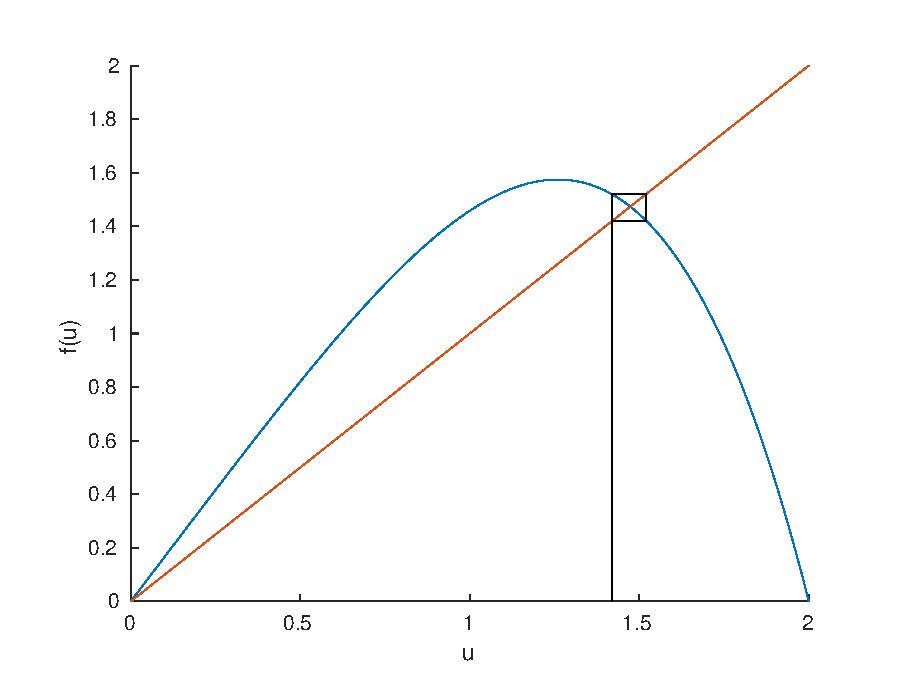
\includegraphics[width=0.7\textwidth]{cicle_2.eps}\\
		{Рис. 3. Нахождение цикла длины 2. $u_1 = 1.418, u_2 = 1.521, r = 0.2083$}
	\end{center}
	{Теперь рассмотрим исходную систему при k = 3:}
	\[ \begin{cases}
	f^{(3)}(u) = u\\
	\frac{df^{(3)}(u)}{du} = 1.
	\end{cases}\]
	{Решив данную систему численно, опять же, с помощью функции MatLab solve, получим пару действительных решений данной системы, однако они будут отрицательными, что, в свою очередь, не удовлетворяет условиям задачи. Из этого делаем вывод, что цикла длины 3 у данной системы нет.}
	{\subsection{Расчет показателя Ляпунова}}
	{\textbf{Определение 2.11.} Пусть $f: \mathds{R} \rightarrow \mathds{R}$--- гладкое отображение. Показателем Ляпунова траектории $u_1,u_2,\ldots,u_n,\ldots$ называется величина:}
	\[ h(u_1) = \lim_{n\to\infty}\frac{ln|f^{'}(u_1)| + ln|f^{'}(u_2)| + \ldots + ln|f^{'}(u_n)|}{n},\]
	{если этот предел существует.}
	{Построим график зависимости показателя Ляпунова от значений параметра $r$. Для этого возьмем начальное приближение $u_0 = 0.01$ и сетку по $r$ c шагом $\delta r = 0.005$ и $n = 1000$ для каждой итерации по $r$. Результат приведен на рис.3.}
	\begin{center}
		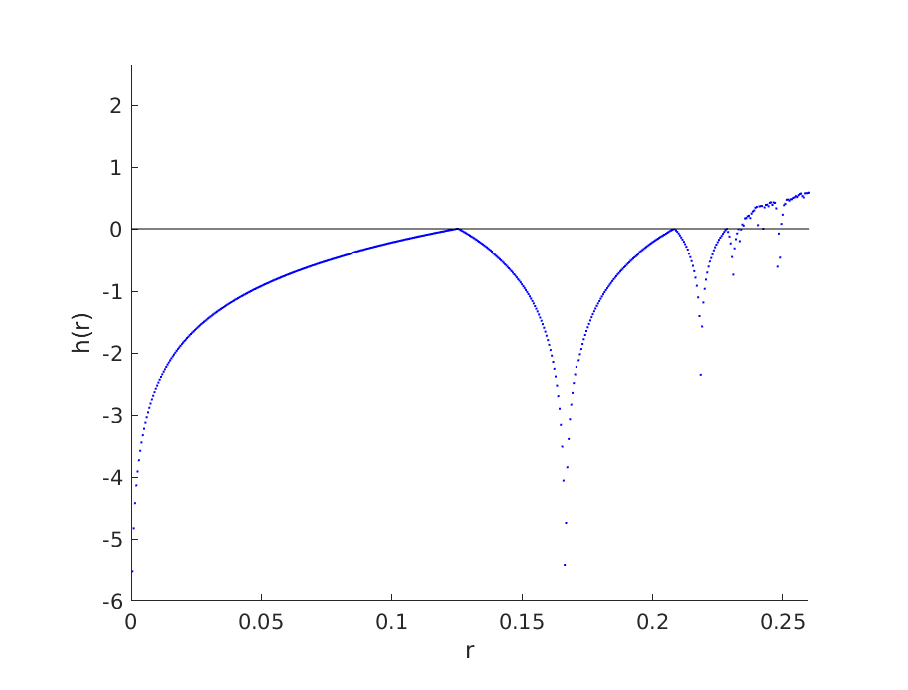
\includegraphics[width=0.7\textwidth]{lapunov_1.eps}\\
		{Рис. 4. График зависимости показателя Ляпунова от $r$.}
	\end{center}
	{Показатель Ляпунова является характеристикой поведения по начальным данным траектории. Если он больше нуля, то близкие траектории разбегаются в системе наблюдается хаотическое поведение. В противном случае расстояние между близкими траекториями уменьшается от итерации к итерации. По рис. 3 видно, что в нашей системе есть хаотическое поведение --- показатель Ляпунова может быть положительным. Так же виден интервал, когда показатель Ляпунова меньше нуля. Он соответствует циклу с небольшим периодом.}
	\newpage
	{\vspace*{-2cm} \hspace*{-1cm}\section{Исследование системы (\ref{eq:ref2})} }
	{Теперь перейдем к исследования системы (2):}
	\[ u_{t+1} = ru_t(8 - u_{t-1}^3), \quad 0 < u_t < 2 \]
	{Системы такого вида называются системами с запаздыванием. Перепишем эту систему в следующем виде, чтобы избавится от запаздывания:}
	\[\begin{cases}
	u_{t+1} = f(u_t,v_t) = ru_t(8 - v_t^3),\\
	v_{t + 1} = g(u_t, v_t) = u_t.
	\end{cases} \]
	{Далее будем исследовать эту систему.}
	\newline
	{\subsection{Неподвижные точки системы (2)}}
	{\textbf{Определение 3.1.} Точка $u^* \in \mathds{R}$ называется неподвижной точкой системы (2) если $f(u^*, u^*) = u^*.$}
	\newline
	{В терминах измененной системы без запаздывания получается, что для нахождения неподвижных точек необходимо решить систему:}
	\[ \begin{cases}
	f(u, v) = u,\\
	g(u,v) = v.
	\end{cases} \]
	{Что эквивалентно системе:}
	\[\begin{cases}
	 ru(8 - u^3) = u,\\
	 v = u.
	\end{cases} \]
	{Таким образом, видно, что у данной системы будут такие же неподвижные точки, как у системы (1) с точностью до добавления второй координаты. Итак, исходная система будет иметь три неподвижные точки, а именно: $a = (0,0), b = ((\frac{8r - 1}{r})^{1/3}, (\frac{8r - 1}{r})^{1/3})$}
	\newline
	{\subsection{Исследование характера неподвижных точек}}
		\begin{theorem}
		{ Пусть дана динамическая система с дискретным временем: $u_{t + 1} = f(u_t),$ где $u_t \in \mathds{R}^n, t \in \mathds{N}, f$--- гладкое отображение из $\mathds{R}^n$ в $\mathds{R}^n$. Тогда неподвижная точка $u^*$ асимптотически устойчива, если все собственные значения $\lambda_1, \lambda_2, \ldots, \lambda_n$ матрицы Якоби функции $f(u),$ вычисленные в точке $u^*$ таковы, что $|\lambda_i| < 1, i =1,\ldots,n.$ Если хотя бы одно собственное значение $\lambda_i$ таково, что $|\lambda_i| > 1$ то неподвижная точка $u^*$ неустойчива.}
	\end{theorem}
	{Выпишем матрицу Якоби для данной системы функций:}
	\[ J(u,v) = \begin{pmatrix}
	\frac{\partial f}{\partial u}& \frac{\partial f}{\partial v} \\
	\frac{\partial g}{\partial u}& \frac{\partial f}{\partial v}
	\end{pmatrix} = \begin{pmatrix}
	r(8 - v^3)& -3ruv^2 \\
	1 & 0
	\end{pmatrix} \]
	\begin{itemize}
		\item [1)]{Рассмотрим точку a = (0,0). Подставив ее в матрицу Якоби и найдя собственные значения, получим: $\lambda_1 = 0, \lambda_2 = 8r.$ При $r < 1/8$ точка а будет асимптотически устойчивой. При $r > 1/8$ --- неустойчива.}
		\item [2)]{Рассмотрим точку $ b = ((\frac{8r - 1}{r})^{1/3}, (\frac{8r - 1}{r})^{1/3}).$ Подставив ее в матрицу Якоби и найдя собственные значения, получим: $\lambda_1 = \frac{1 - i\sqrt{96r - 13}}{2}, \lambda_2 = \frac{1 + i\sqrt{96r - 13}}{2}.$ $|\lambda_1| = |\lambda_2| = \sqrt{24r - 3}.$ Решив неравенства  $0 < \sqrt{24r - 3} < 1$ получим, что точка b асимптотически устойчива при $r \in (\frac{1}{8}, \frac{1}{6})$, при $r = \frac{1}{6}, |\lambda_{1,2}| = 1$ и поэтому нужны дополнительные исследования, и не устойчива в остальных случаях.}
	\end{itemize}
 	{\subsection{Бифуркация Неймарка-Сакера}}
 	{\textbf{Определение 3.2.} Бифуркация положения равновесия в системе:}
 	\[ u \rightarrow f(u,r), u = (u_1, u_2) \in \mathds{R}^2, r \in \mathds{R},\] 
 	{соответствующая появлянию собственных значений $|\lambda_1| = |\lambda_2| = 1, \lambda_1 = \overline{\lambda_2},$ называется бифуркацией Неймарка-Сакера или дискретной бифуркацией Хопфа.}
 	\newline
 	{Исходя из результатов предыдущего пункта, можно сделать вывод, что существует $r$ при котором бифуркация Неймарка-Сакера существует. При этом, значение параметра $r$ при котором она существует равна $r = 1/6.$}
 	\newline
 	{Рассмотрим точку $((\frac{8r - 1}{r})^{1/3}, (\frac{8r - 1}{r})^{1/3}) = (1.418, 1.418)$, и построим бифуркацию в окрестностях этой точки:}
 	\begin{center}
 		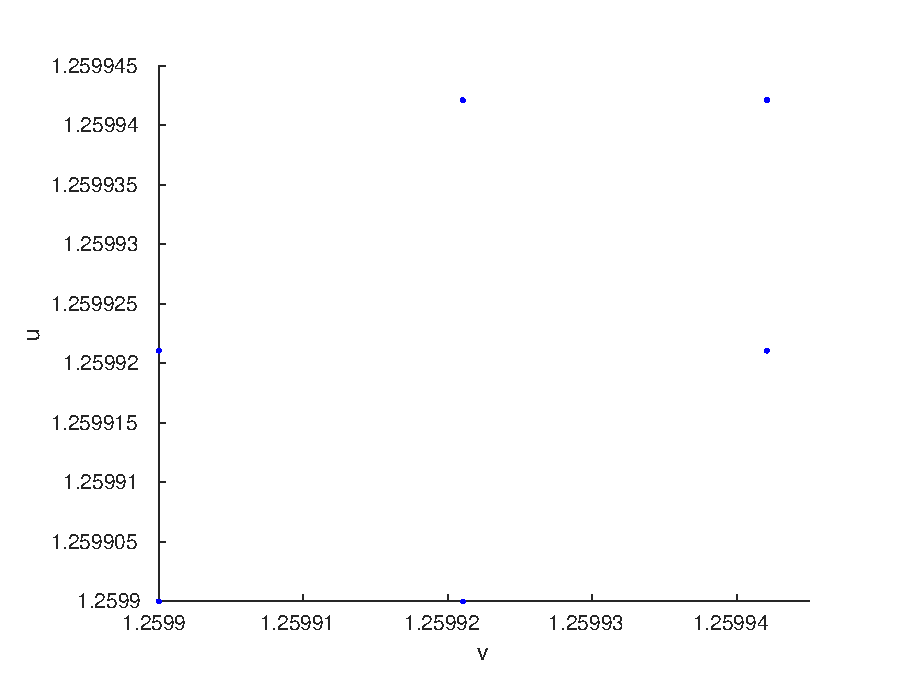
\includegraphics[width=0.7\textwidth]{bifur_ns.eps}\\
 		{Рис. 5. Поведение траекторий в неподвижной точке (1.2599, 1.2599) при $r = 1/6, n = 1000.$}
 	\end{center}
 	\newpage
 	\begin{center}
 		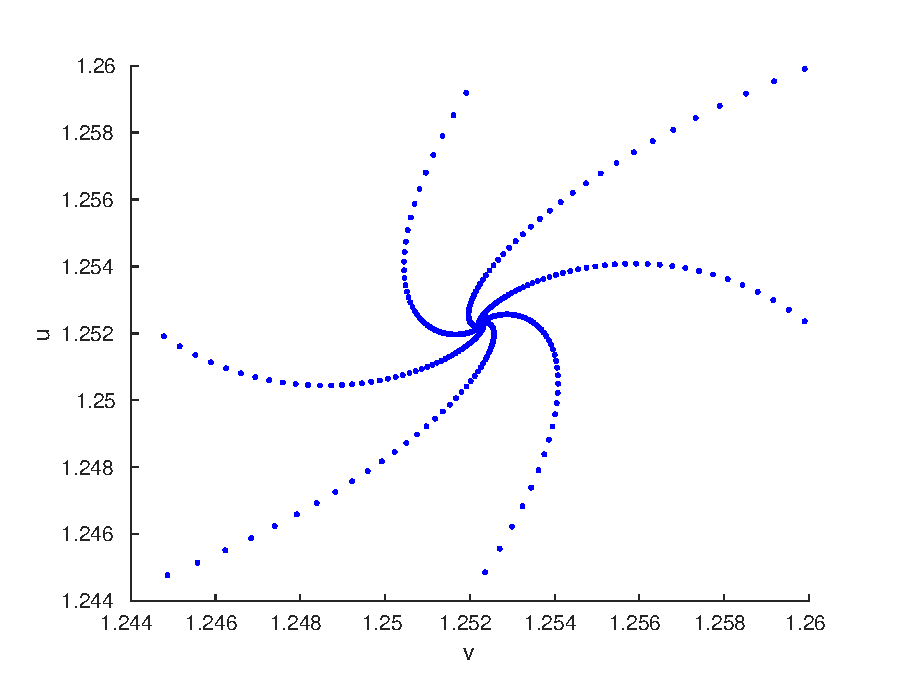
\includegraphics[width=0.7\textwidth]{bifur_ns_1.eps}\\
 		{Рис. 6. Поведение траекторий в окрестности неподвижной точки (1.2599, 1.2599) при $r = 1/6 - 1/1000, n = 1000$.}
 	\end{center}
 	\begin{center}
 		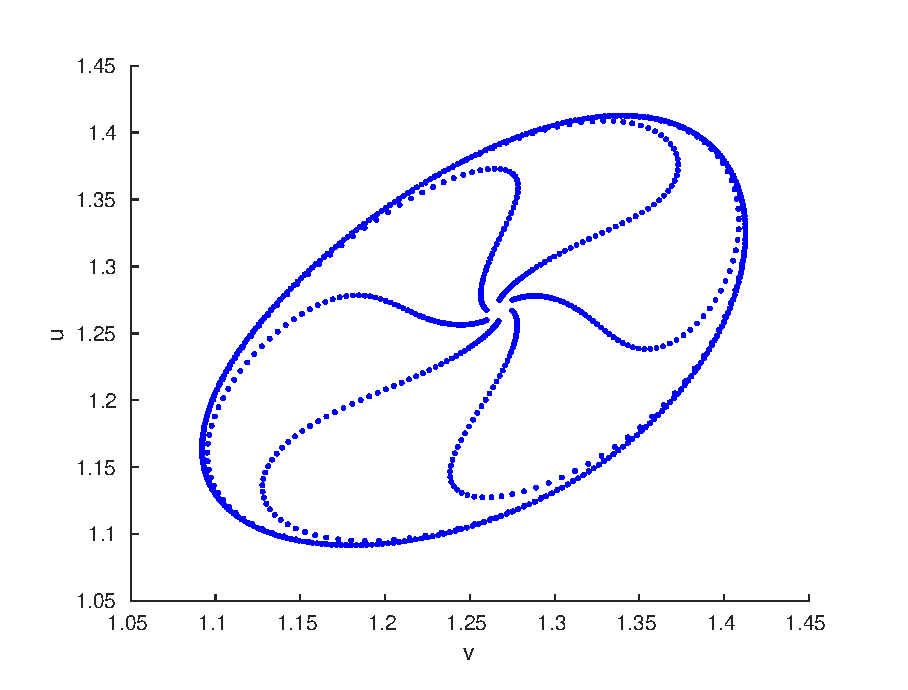
\includegraphics[width=0.7\textwidth]{bifur_ns_2.eps}\\
 		{Рис. 7. Поведение траекторий в окрестности неподвижной точки (1.2599, 1.2599) при $r = 1/6 + 1/1000, n = 1000$.}
 	\end{center}
 	\newpage
 	{\section{Список литературы}}
 	{\hspace*{-0.6cm}[1] Братусь А.С., Новожилов А.С., Платонов А.П. Динамические системы и модели биологии. }
 	
\end{document}